\section{Lecture 3: Dot Product}
\begin{itemize}
    \item Let $\vec{v}=\begin{bmatrix}
        v_1\\v_2\\v_3
    \end{bmatrix}$, and $\vec{w}=\begin{bmatrix}
        w_1\\w_2\\w_3
    \end{bmatrix}$, then the dot product of two vectors in $\mathbb{R}^3$ is:
    \begin{equation}
        \vec{v}\cdot\vec{w} = v_1w_1+v_2w_2+v_3w_3
        \label{eq:}
    \end{equation}
    also sometimes known as the \textbf{scalar product}, which comes from the fact that the dot product gives a scalar quantity. This is a \textit{definition}.
    \item There are a few properties of dot products:
    \begin{itemize}
        \item The distributive property: $\vec{v} \cdot (\vec{w}+\vec{z})=\vec{v}\cdot\vec{w}+\vec{v}\cdot\vec{z}$
        \begin{prooof}
            Let $\vec{v}=\begin{bmatrix}
                v_1\\v_2\\v_3
            \end{bmatrix}$, $\vec{w}=\begin{bmatrix}
                w_1\\w_2\\w_3
            \end{bmatrix}$, and $\vec{z}=\begin{bmatrix}
                z_1\\z_2\\z_3
            \end{bmatrix}$. Then:
            \begin{align}
                \vec{v}\cdot(\vec{w}+\vec{z}) &= \begin{bmatrix}
                    v_1\\v_2\\v_3
                \end{bmatrix} \cdot \left(\begin{bmatrix}
                    w_1\\w_2\\w_3
                \end{bmatrix}+\begin{bmatrix}
                    z_1\\z_2\\z_3
                \end{bmatrix}\right) \\ 
                &= \begin{bmatrix}
                    v_1\\v_2\\v_3
                \end{bmatrix} \cdot \begin{bmatrix}
                    w_1+z_1\\w_2+z_2\\w_3+z_3
                \end{bmatrix} \\ 
                &=
                \begin{bmatrix}
                    v_1(w_1+z_1) \\ 
                    v_2(w_2+z_2) \\ 
                    v_3(w_3+z_2) \\ 
                \end{bmatrix} \\ 
                &= \vec{v}\cdot\vec{w}+\vec{v}\cdot\vec{z}
                \label{eq:}
            \end{align}
        \end{prooof}
        \item The commutative property: $\vec{v}\cdot\vec{w} = \vec{w}\cdot\vec{v}$.
        \item Associative: $c(\vec{v}\cdot\vec{w})=(c\vec{v})\cdot\vec{w}=\vec{v}\cdot(c\vec{w})$
    \end{itemize}
    \item There is an important connection between the length of a vector and the dot product. Recall that:
    \begin{equation}
        \lVert \vec{v} \rVert = \sqrt{v_1^2+v_2^2+v_3^2}
        \label{eq:}
    \end{equation}
    We can square this to notice that the RHS is just the dot product of a vector with itself:
    \begin{equation}
        \lVert \vec{v} \rVert^2 = v_1^2+v_2^2+v_3^2 = \vec{v}\cdot\vec{v}
        \label{eq:}
    \end{equation}
    Thus:
    \begin{equation}
        \lVert \vec{v} \rVert = \sqrt{\vec{v}\cdot\vec{v}}
        \label{eq:}
    \end{equation}
    \begin{example}
        Suppose we wish to find the angle between two vectors $\vec{v}$ and $\vec{w}$. Traditionally, we may want to complete the triangle by drawing the vector $\vec{w}-\vec{v}$.
        \begin{center}
            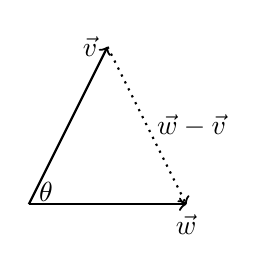
\begin{tikzpicture}
                \draw[thick,->] (0,0) node[above right,yshift=-0.1cm] {$\theta$} -- (2,0) node[below] {$\vec{w}$};
                \draw[thick,->] (0,0) -- (1,2) node[left] {$\vec{v}$};
                \draw[thick,dotted,->] (1,2) -- (2,0) node[midway,right] {$\vec{w}-\vec{v}$};
            \end{tikzpicture}
        \end{center}
        We can then write:
        \begin{align}
            \lVert \vec{w}-\vec{v} \rVert^2 &= (\vec{w}-\vec{v})\cdot (\vec{w}-\vec{v}) \\ 
            &= \vec{w}\cdot\vec{w}-2\vec{v}\cdot\vec{w}+\vec{v}\cdot\vec{v} \\ 
            &=\lVert \vec{w} \rVert ^2 + \lVert \vec{v} \rVert^2-2\vec{w}\cdot\vec{v}
        \end{align}
        This resembles the cosine law:
        \begin{equation}
            \lVert \vec{w}-\vec{v}\rVert^2 = \lVert \vec{w}\rVert^2+\lVert \vec{v} \rVert^2 - 2\lVert \vec{w}\rVert \lVert \vec{v} \rVert \cos\theta
            \label{eq:}
        \end{equation}
        By comparison, we can conclude that:
        \begin{equation}
            \vec{w}\cdot\vec{v} = \lVert \vec{v} \rVert \lVert \vec{w} \rVert \cos\theta
            \label{eq:}
        \end{equation}
        This is \textit{not} the definition of the dot product, but only a geometric interpretation of it. We can solve for $\cos\theta$ to be in this case:
        \begin{equation}
            \cos\theta = \frac{\vec{w}\cdot\vec{v}}{\lVert \vec{w} \rVert \lVert \vec{v} \rVert}
            \label{eq:}
        \end{equation}
    \end{example}
    \item Note that the sign of the dot product tells us some important information about the angle $\theta$. For example, if we know that $\vec{v}\cdot\vec{w}>0$, then this is true if and only if $0 \le \theta < \pi/2$ (or in other words, acute). Similarly, $\vec{v}\cdot\vec{w}=0 \iff \theta=\pi/2$ and $\vec{v}\cdot\vec{w}>0 \iff \theta>\pi/2$
    \begin{theorem}
        The triangle inequality tells us:
        \begin{equation}
            \lVert \vec{v}+\vec{w} \rVert \le \lVert \vec{v} \rVert + \lVert \vec{w} \rVert
            \label{eq:}
        \end{equation}
    \end{theorem}
    \item We can visualize the triangle inequality intuitively by drawing a diagram:
    \begin{center}
        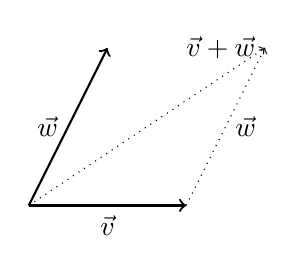
\begin{tikzpicture}
            \draw[thick,->] (0,0) -- (2,0) node[midway,below] {$\vec{v}$};
            \draw[thick,->] (0,0) -- (1,2) node[midway,left] {$\vec{w}$};
            \draw[dotted,->] (2,0) -- (3,2) node[midway,right] {$\vec{w}$};
            \draw[dotted,->] (0,0) -- (3,2) node[left] {$\vec{v}+\vec{w}$};
        \end{tikzpicture}
    \end{center}
    and we can intuitively see that $\vec{v}+\vec{w}$ has to be have a smaller length than the sum of the two lengths of $\vec{v}$ and $\vec{w}$. However, we need to do this algebraically:
    \begin{prooof}
        We write:
        \begin{align}
            \lVert \vec{v}+\vec{w} \rVert ^2 &= (\vec{v}+\vec{w})\cdot(\vec{v}+\vec{w}) \\
            &= \vec{v}\cdot\vec{v} + 2\vec{v}\cdot\vec{w}+\vec{w}\cdot\vec{w} \\ 
            &= \lVert \vec{v}\rVert^2+ \lVert \vec{w} \rVert^2+2\lVert\vec{v}\rVert\lVert\vec{w}\rVert\cos\theta
        \end{align}
        To get the inequality, we can replace $\cos\theta$ by its least upper bound. Then:
        \begin{align}
            \lVert \vec{v}+\vec{w} \rVert^2 &\le \lVert \vec{v} \rVert^2+\lVert \vec{w} \rVert^2+2\lVert\vec{v}\rVert\lVert\vec{w}\rVert (1) \\
            &\le \left(\lVert\vec{v}\rVert+\lVert\vec{w}\rVert\right)^2
        \end{align}
        Taking the root of both sides (since none of the magnitudes can be negative), we are then able to prove the triangle inequality.
    \end{prooof}
    \begin{theorem}
        The \textbf{Cauchy-Schwarz-Bunakowsky Inequality} relates the absolute magnitude of the dot product:
        \begin{equation}
            |\vec{v}\cdot\vec{w} \le \lVert\vec{v}\rVert\lVert\vec{w}\rVert
            \label{eq:}
        \end{equation}
        
    \end{theorem}
\end{itemize}